\begin{figure}[hbtp]
  \centering
  \subfigure{
    \label{fig:rak-hashtable--all}
    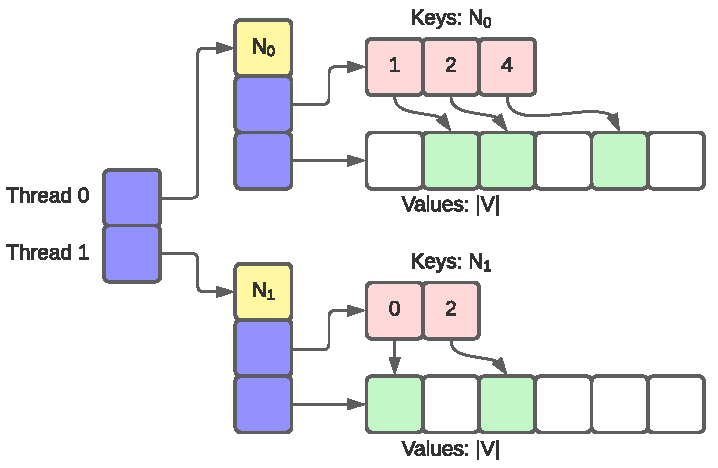
\includegraphics[width=0.88\linewidth]{out/rak-hashtable.pdf}
  } \\[-2ex]
  \caption{Illustration of collision-free per-thread hashtables with well separated memory addresses (Far-KV) for two threads. Each hashtable comprises a keys vector, a values vector (of size $|V|$), and a key count ($N_0$/$N_1$). The value corresponding to each key is stored/accumulated at the index indicated by the key. As the key count of each hashtable is updated independently, we allocate it separately on the heap to avoid false cache sharing \cite{sahu2023gvelouvain}.}
  \label{fig:rak-hashtable}
\end{figure}
